\documentclass[12pt,a4paper]{article}
\synctex=1
\usepackage[utf8]{inputenc}
\usepackage[margin=1cm]{geometry}
\usepackage{graphicx}
%\usepackage{verbatim}
\usepackage{listings}
\usepackage{textcomp}
\usepackage{courier}
\usepackage{libertine}
\usepackage{pgfornament}
\usepackage{eso-pic}
\usepackage[hangul]{kotex}
\linespread{1.3}

\title{
	\centering
	\pgfornament[width=12cm,color=teal]{84}\\
	\vspace{1cm}
	\fontsize{50}{50} \selectfont {컴퓨터 그래픽스 입문}\\
		\pgfornament[width=12cm,color=teal]{88}\\
	\vfill}
\author{
	\LARGE
	\begin{tabular}{rl}
		\hline
		학번 : & 2016110056\\ 
		학과 : & 불교학부 \\
		이름 : & 박승원\\
		날짜 : & \today\\
		\hline
	\end{tabular}\vspace{2cm}
	\\

\includegraphics[width=0.5\textwidth]{logo.jpg}
	}
\date{}


\begin{document}
\maketitle
\pagenumbering{gobble}
\noindent
\lstset{language=C++, columns=flexible, tabsize=4, frame=shadowbox, showstringspaces=false, breaklines=true, upquote=true, basicstyle=\normalsize}
\newpage
\section*{Lab 9. Viewing}
	
\begin{verbatim}
Use 'keyboard' to change your view like mouse controls do in the example code.
	
	- 'Q / E' : rotation (imagine that you are a game character of a FPS game. 
				Q turns your head left, E turns your head right) (2pt)
	- 'W' : move forward to the object (2pt)
	- 'S' : move backward from the object (2pt)
	- 'A' : side step left (imagine one more time that you are a FPS 
			game character) (2pt)
	- 'D' : side step right (imagine one more time that you are a FPS 
			game character) (2pt)

머리를 돌리는 것은 Y축을 기준으로 회전하는 것과 같고, 가까이 다가가는 것과 멀어지는 것은 scale과 같고, 좌우로 움직이는 것은 translation과 같다.
기존에 구현했던 callback을 조금 고치는 것으로 가능했다.
KeyBindMatrix는 메인화일에서 물체들을 변환한다.
또한 프로젝션 매트릭스를 이용해야 접근과 멀어짐, 좌우 회전이 더욱 실감난다.
\end{verbatim}

\begin{lstlisting}
	void key_callback(GLFWwindow* window, int key, int scancode, int action, int mods) 
	{// && action == GLFW_PRESS) 
		switch(key) {
			case GLFW_KEY_A:
			KeyBindMatrix = m.gltranslate(-STEP, 0, 0) * KeyBindMatrix; break;
			case GLFW_KEY_DOWN:
			KeyBindMatrix = m.gltranslate(0, -STEP, 0) * KeyBindMatrix; break;
			case GLFW_KEY_D:
			KeyBindMatrix = m.gltranslate(STEP, 0, 0) * KeyBindMatrix; break;
			case GLFW_KEY_UP:
			KeyBindMatrix = m.gltranslate(0, STEP, 0) * KeyBindMatrix; break;
			case GLFW_KEY_W:
			KeyBindMatrix = m.gltranslate(0, 0, STEP) * KeyBindMatrix; break;
			case GLFW_KEY_S:
			KeyBindMatrix = m.gltranslate(0, 0, -STEP) * KeyBindMatrix; break;
			
			//	case GLFW_KEY_W: KeyBindMatrix = m.glrotateX(STEP) * KeyBindMatrix; break;
			//	case GLFW_KEY_A: KeyBindMatrix = m.glrotateY(-STEP) * KeyBindMatrix; break;
			//	case GLFW_KEY_S: KeyBindMatrix = m.glrotateX(-STEP) * KeyBindMatrix; break;
			//	case GLFW_KEY_D: KeyBindMatrix = m.glrotateY(STEP) * KeyBindMatrix; break;
			case GLFW_KEY_Q: KeyBindMatrix = m.glrotateY(-STEP) * KeyBindMatrix; break;
			case GLFW_KEY_E: KeyBindMatrix = m.glrotateY(STEP) * KeyBindMatrix; break;
			
			case GLFW_KEY_SPACE: KeyBindMatrix.E(); break;
			
			case GLFW_KEY_J: camera_x -= STEP; break;
			case GLFW_KEY_K: camera_y -= STEP; break;
			case GLFW_KEY_L: camera_x += STEP; break;
			case GLFW_KEY_I: camera_y += STEP; break;
		}
	}
\end{lstlisting}
\lstinputlisting[caption=main]{src/val4.cpp}

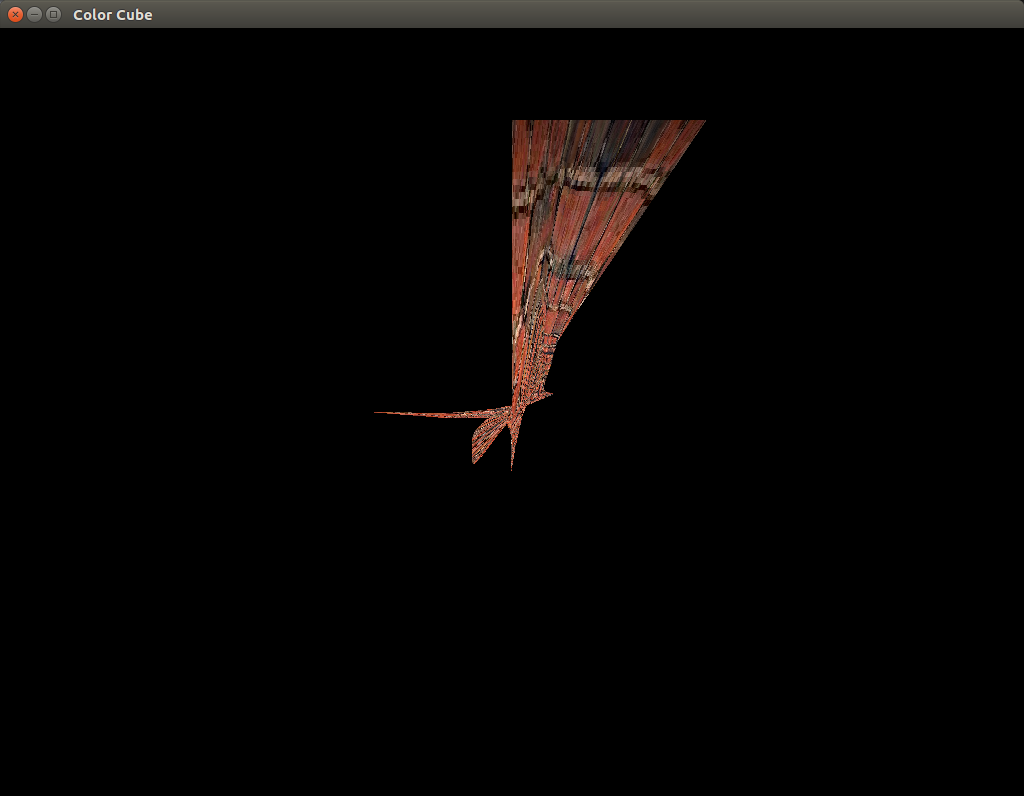
\includegraphics[width=\textwidth]{1.png}	

\end{document}
